%-------------------------------------------------------------------------------

% This file is part of Code_Saturne, a general-purpose CFD tool.
%
% Copyright (C) 1998-2011 EDF S.A.
%
% This program is free software; you can redistribute it and/or modify it under
% the terms of the GNU General Public License as published by the Free Software
% Foundation; either version 2 of the License, or (at your option) any later
% version.
%
% This program is distributed in the hope that it will be useful, but WITHOUT
% ANY WARRANTY; without even the implied warranty of MERCHANTABILITY or FITNESS
% FOR A PARTICULAR PURPOSE.  See the GNU General Public License for more
% details.
%
% You should have received a copy of the GNU General Public License along with
% this program; if not, write to the Free Software Foundation, Inc., 51 Franklin
% Street, Fifth Floor, Boston, MA 02110-1301, USA.

%-------------------------------------------------------------------------------

\section{Solution for case2}
This case corresponds to a new study, in which there will be three calculation
cases (cases 2, 3 and 4).
We can create one case in a single \texttt{code\_saturne create} command and
additional cases can be added later.
To test this functionality, first create the study directory, with case
subdirectory \texttt{case2}, as below:\\
\fbox{\begin{minipage}{\textwidth}\texttt{\\
\$ {\color{blue}code\_saturne create -s full\_domain -c case2}\\
\$ cd full\_domain
}\end{minipage} }

Go to the \texttt{DATA} directory in \texttt{case2}, open a new case and select
the meshes to use.

Click on the heading {\itshape Calculation environment} then on the {\itshape Meshes selection} item.
In this case, you must add three meshes which have to be joined.

In order to join the three meshes, you must add a selection criteria in the
box {\itshape Selection criteria}. In this case, only faces of colors 5, 24 and 32
are liable to be joined (different colors can be entered on a single line, separated by comma).

Click on the {\bf +} icon to enter the list of colors to be joined in the
{\itshape Face joining (optional)} item.

\begin{figure}[h!]
\begin{center}
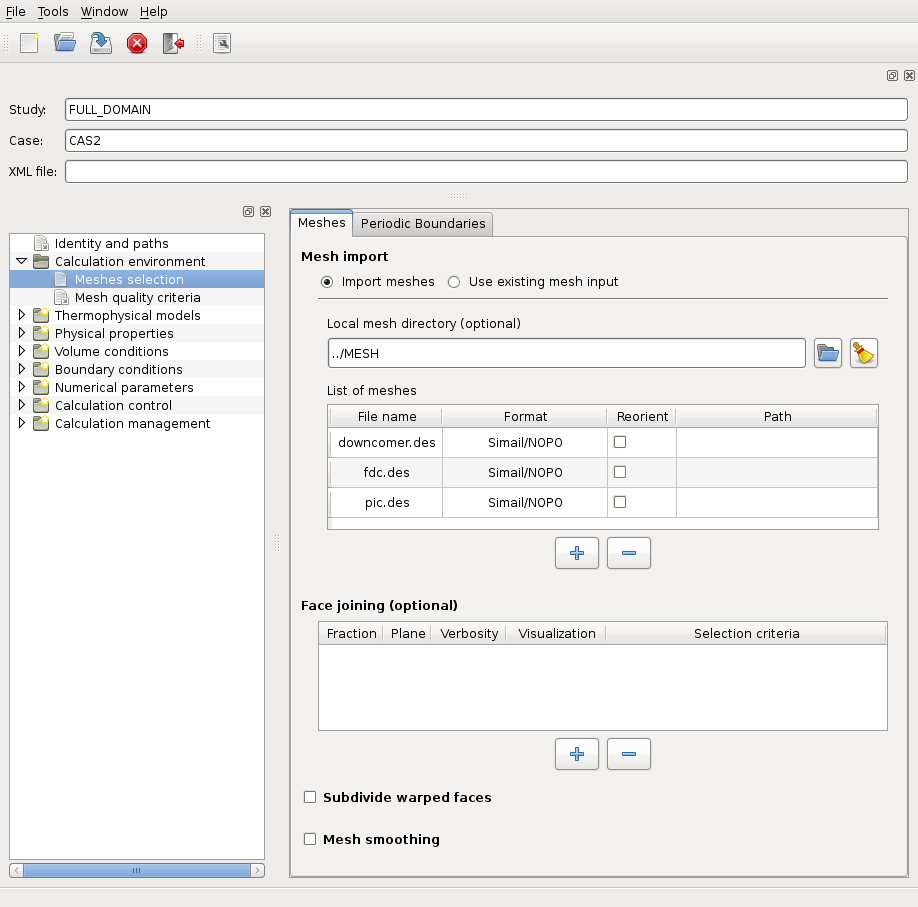
\includegraphics[width=12cm]{case2_V-1}
\caption{Meshes: list of meshes}
\label{fig2_e2}
\end{center}
\end{figure}


\newpage
\begin{figure}[h!]
\begin{center}
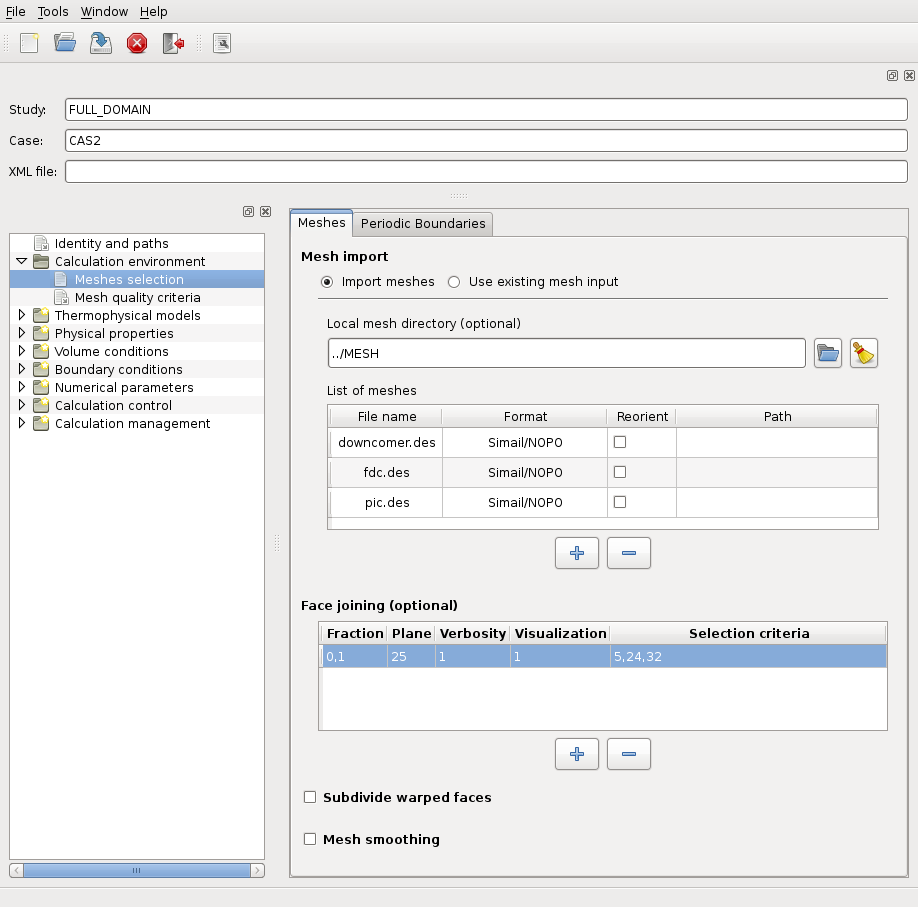
\includegraphics[width=12cm]{case2_V-2}
\caption{Join a Mesh}
\label{fig4_e2}
\end{center}
\end{figure}

\newpage
You can now verify the quality of your mesh.
\begin{figure}[h!]
\begin{center}
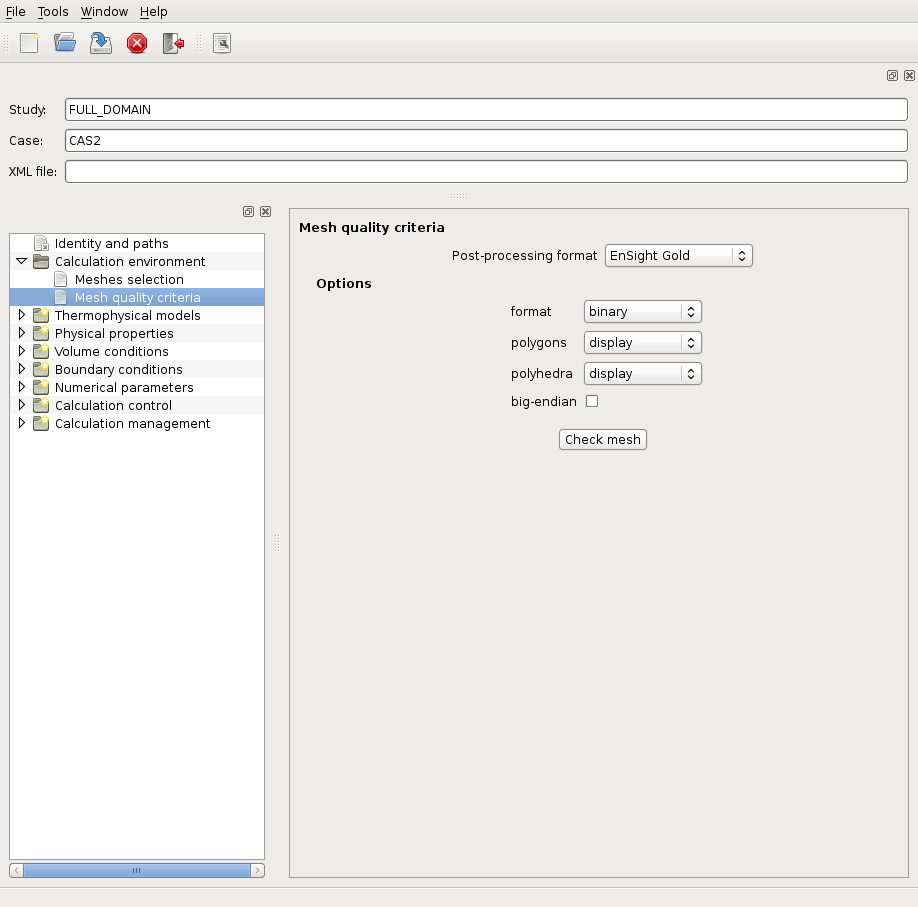
\includegraphics[width=12cm]{case2_V-3}
\caption{Mesh quality criteria}
\label{fig4_e2}
\end{center}
\end{figure}

\newpage
In this case ``Unsteady flow'' must be selected in the
{\itshape Calculation features} item.

\begin{figure}[h!]
\begin{center}
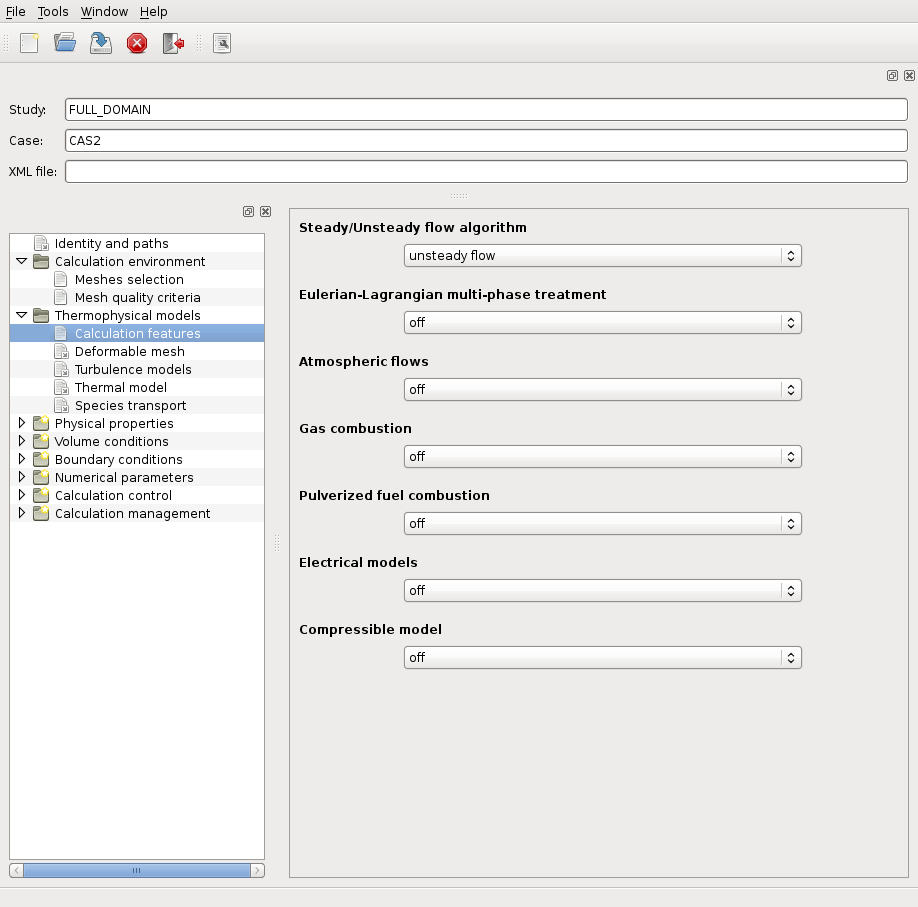
\includegraphics[width=12cm]{case2_V-4}
\caption{Thermophysical models - Analysis features - Unsteady flow}
\label{fig6_e2}
\end{center}
\end{figure}

The rest of the heading {\itshape Thermophysical models} is identical to \texttt{case1}.


\newpage
To add an additional scalar, click on the
{\itshape Species transport} item under the
{\itshape Thermophysical models} heading.

\begin{figure}[h!]
\begin{center}
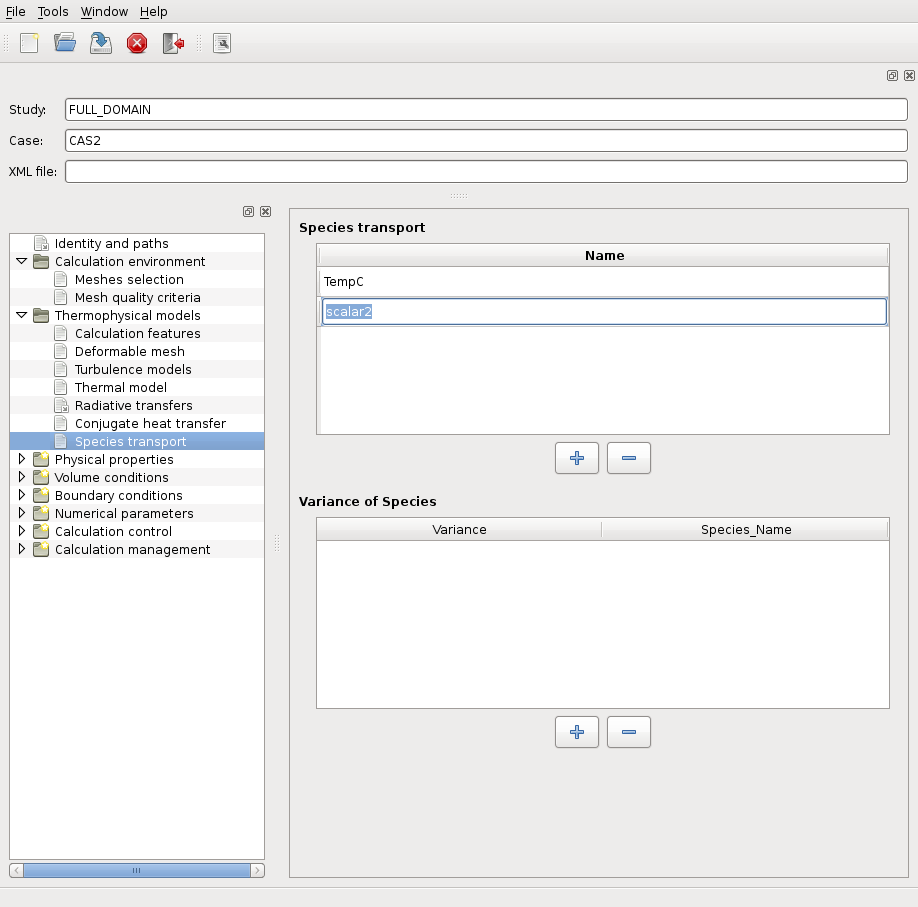
\includegraphics[width=12cm]{case2_V-5}
\caption{Additional scalar}
\label{fig8_e2}
\end{center}
\end{figure}


\newpage
The heading of {\itshape Physical properties} is identical to \texttt{case1}.\\
In the {\itshape Fluid properties} item, still under the heading {\itshape Physical properties},
specify the diffusion coefficient of this new scalar.

Click on the scalar name to highlight it, then enter the value in the box.
In this case, the species diffusion coefficient value is {\bf 0.855} ($\times 10^{-5}\ m^{2}.s^{-1}$)
for the \texttt{scalar2} scalar to solve.

\begin{figure}[h!]
\begin{center}
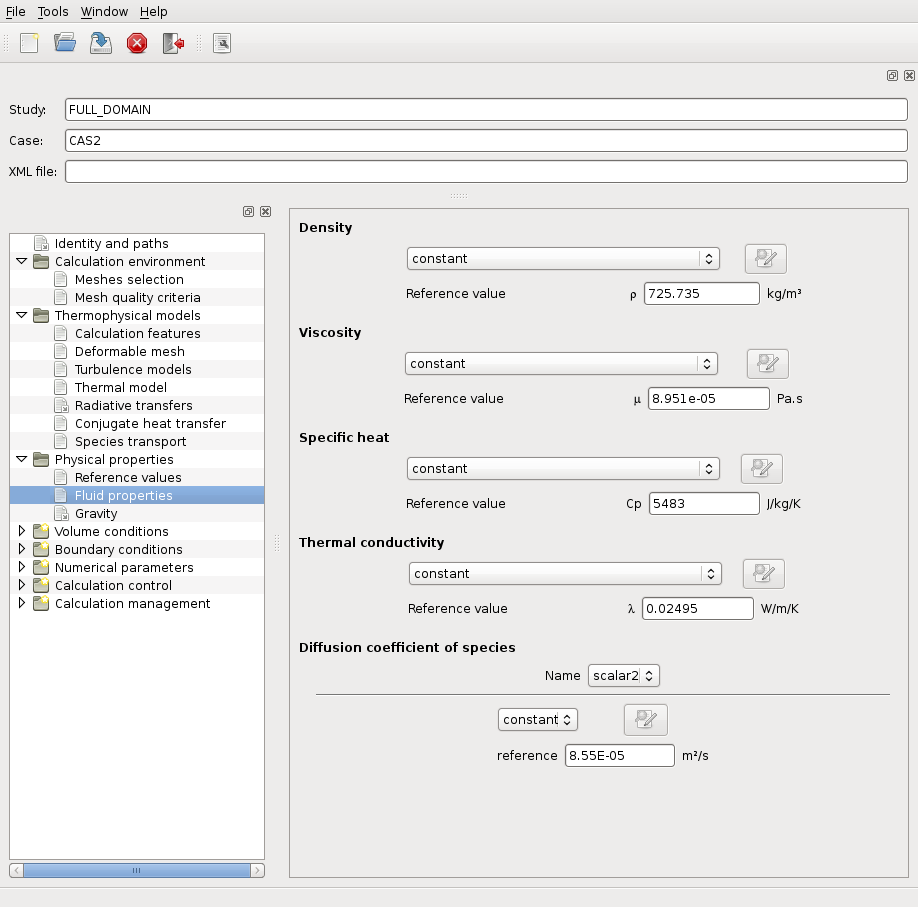
\includegraphics[width=12cm]{case2_V-6}
\caption{Fluid properties}
\label{fig9_e2}
\end{center}
\end{figure}

\newpage
\textbf{Initialization:}\\
To initialize variables at the instant $t=0\ s$, go to the {\itshape Initialization}
item under the heading {\itshape Volume conditions}.

Here the velocity, the thermal scalar and the turbulence can be initialized.
In this case, the default values can be kept: zero velocity, an initial temperature of
{\bf 20}\degresC\  and a turbulence level based on a reference velocity of {\bf 1} ($m.s^{-1}$).
You must also initialize the \texttt{scalar2} species at {\bf 10}\degresC.

Specific zones can be defined with different initializations. In this case, only the
default ``all cells'' is used.
\begin{figure}[h!]
\begin{center}
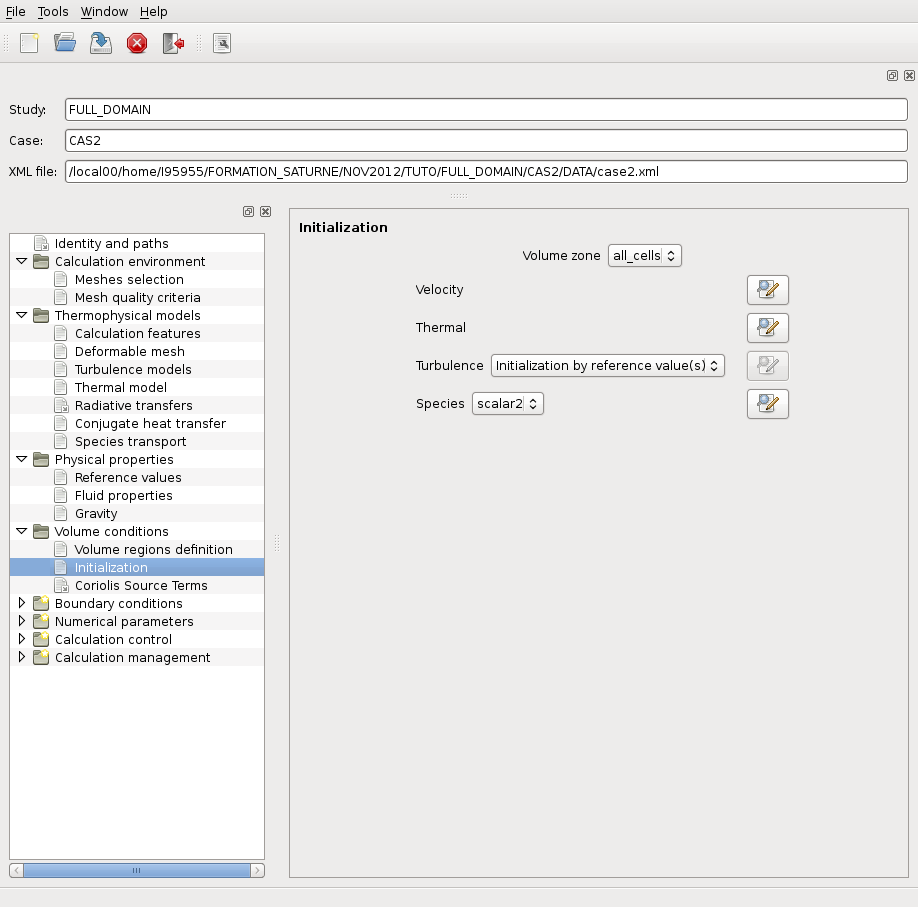
\includegraphics[width=12cm]{case2_V-7}
\caption{Initialization}
\label{fig9_e2}
\end{center}
\end{figure}
\newpage
\begin{figure}[h!]
\begin{center}
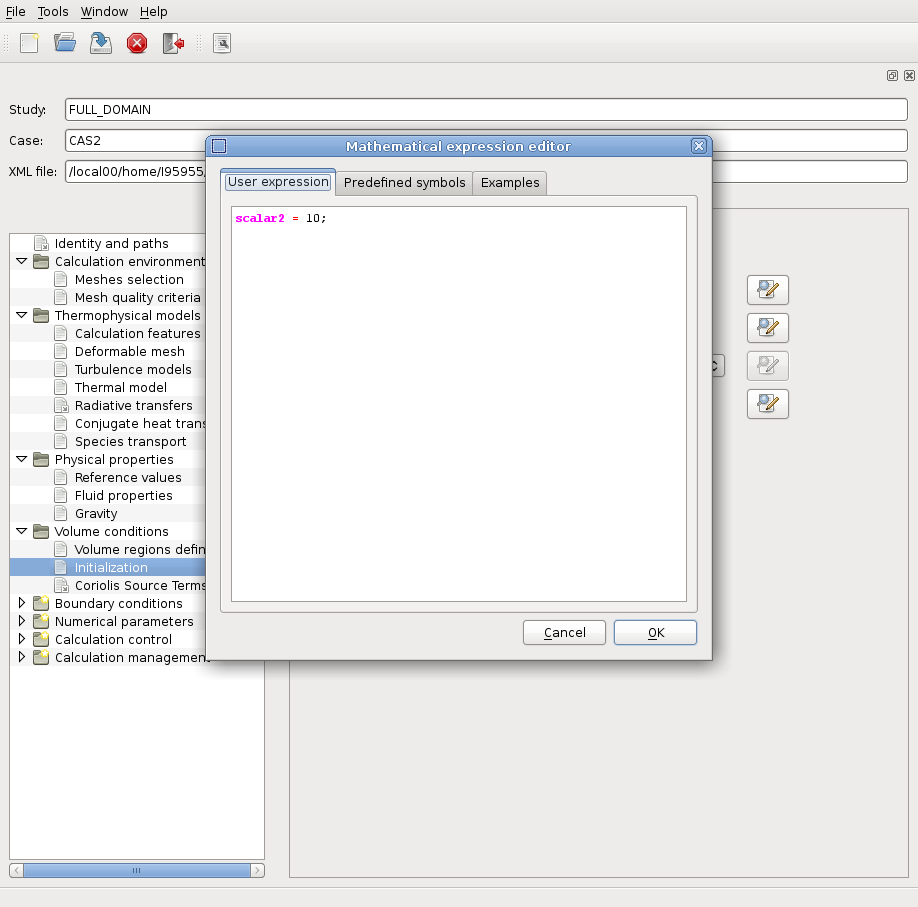
\includegraphics[width=12cm]{case2_V-8}
\caption{Initialization- Species}
\label{fig9_e2}
\end{center}
\end{figure}

\newpage
$\bullet${\bf Create the boundary zones}:\\
The procedure is the same as in case 1, but the colors are different.
Note that colors 5 and 32 have completely disappeared in the joining process
(they are now internal faces and are not considered as boundaries), while some
boundary faces of color 24 remain.

Create the inlet, outlet and symmetry boundary zones with the following colors:\\
\fbox{\begin{minipage}{\textwidth}\texttt{    \\
 - inlet~~~: ''1''\\
 - outlet~~: ''34''\\
 - symmetry: ''8 or 9 or 28 or 29 or 38 or 39''
}\end{minipage} }

\begin{figure}[h!]
\begin{center}
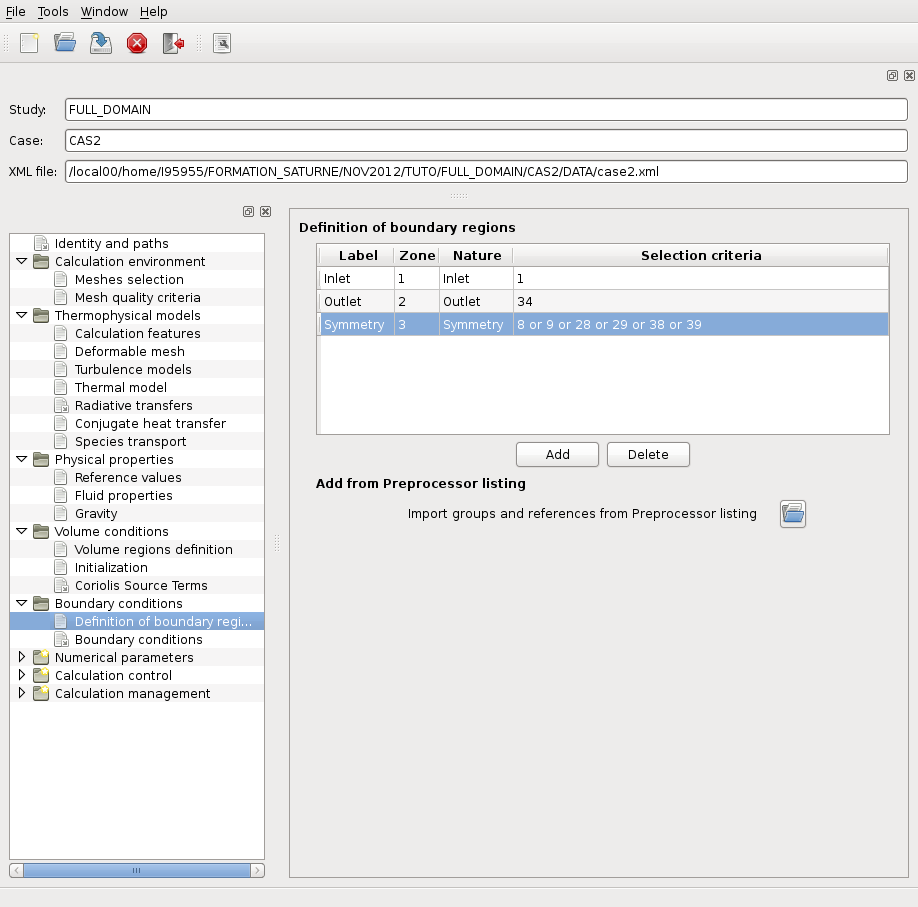
\includegraphics[width=12cm]{case2_V-9}
\caption{Creation of the boundary zones}
\label{fig10_e2}
\end{center}
\end{figure}


\newpage
In this case, different conditions are applied for the walls. Separate
corresponding wall boundary regions must therefore be created, following the
data in the following table.

\begin{center}
\begin{tabular}{|c|c|c|c|}
\hline
Label & Zone & Nature & Selection criteria \\
\hline
\hline
wall\_2 & 5 & wall & 2 or 3 \\
\hline
wall\_3 & 6 & wall & 4 or 7 or 21 or 22 or 23 \\
\hline
wall\_4 & 7 & wall & 6 and y$>$1 \\
\hline
wall\_5 & 8 & wall & 6 and y$\leqslant$1 \\
\hline
wall\_6 & 9 & wall & 31 or 33 \\
\hline
\end{tabular}
\end{center}

The ``wall\_1'' region combines color and geometrical criteria. The associated
character string to enter in the ``Selection criteria'' box\footnote{Note that, due to the joining process,
there are in fact no boundary faces of color 24 with x coordinate outside the
[0.1;0.5] interval. The geometrical criterium is therefore not necessary.
It is presented here to show the capacity of the face selection module.}
 is as follows:\\
\fbox{\begin{minipage}{\textwidth}\texttt{
''24 and 0.1 <= x and 0.5 >= x''
}\end{minipage} }

\begin{figure}[h!]
\begin{center}
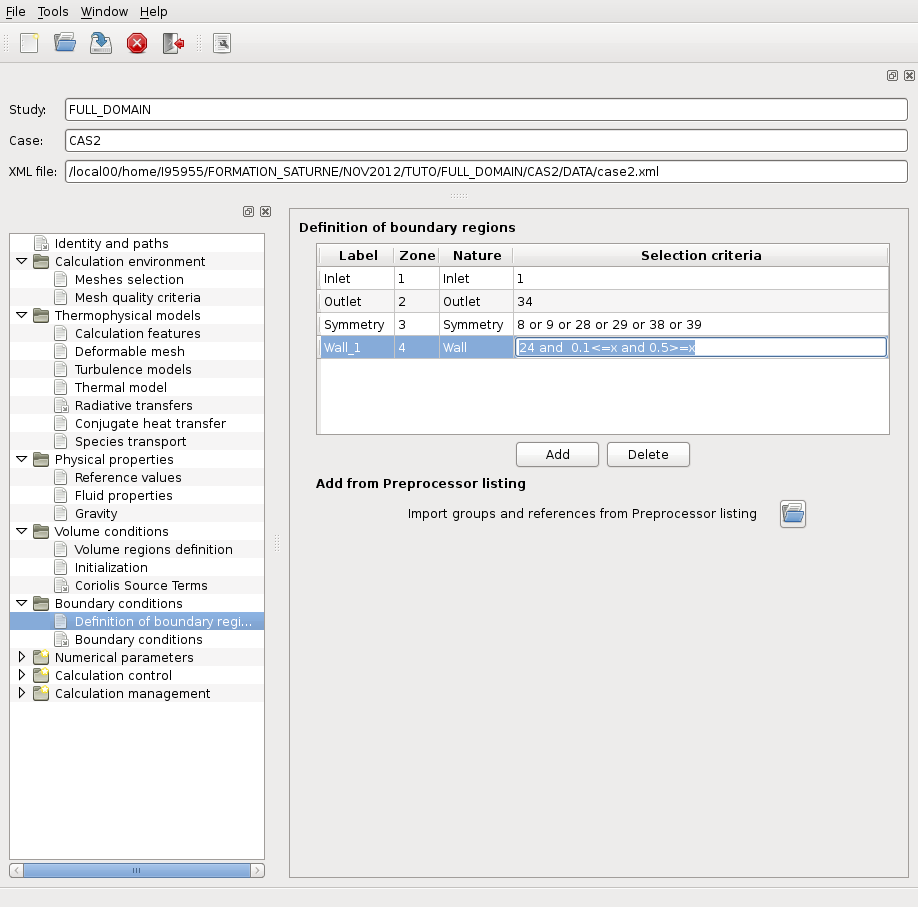
\includegraphics[width=10cm]{case2_V-10}
\caption{Creation of a wall boundary region}
\label{fig11_e2}
\end{center}
\end{figure}


\newpage
Define the other wall boundary zones. The faces of color 6 have to be divided in
two separate zones, based on a geometrical criterium on $y$.

\begin{figure}[h!]
\begin{center}
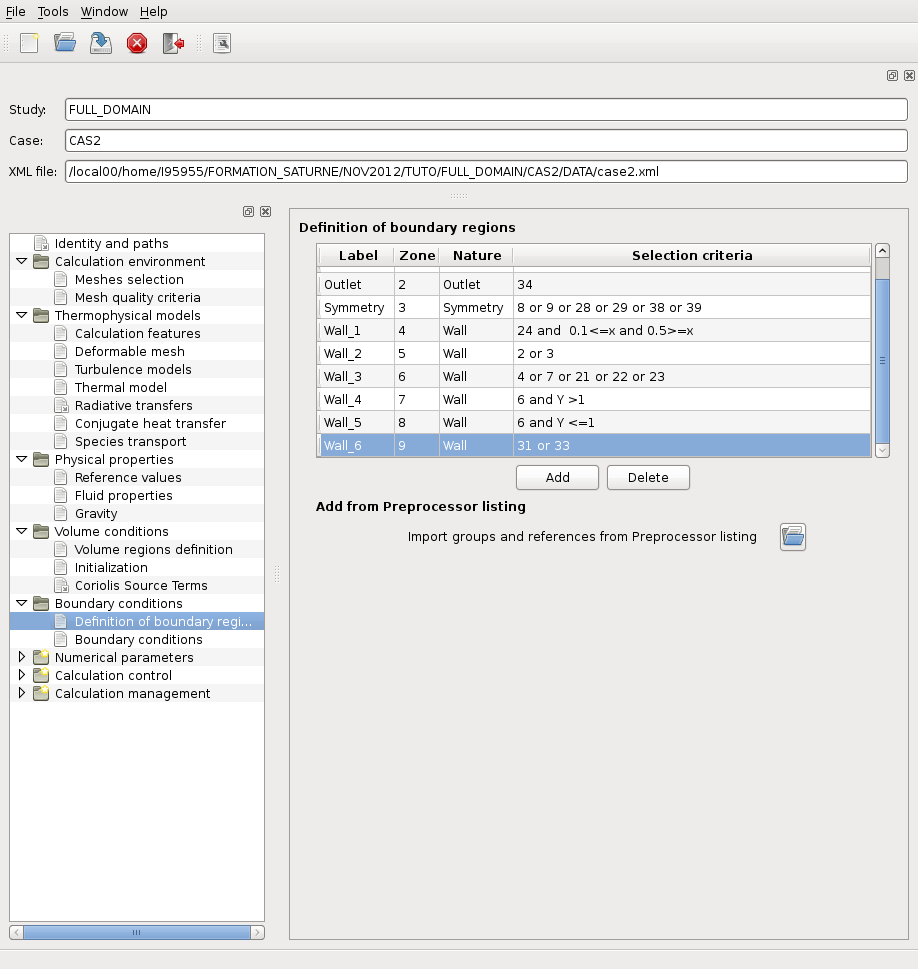
\includegraphics[width=9cm]{case2_V-11}
\caption{Creation of wall boundary regions}
\label{fig152_e2}
\end{center}
\end{figure}


\newpage
The dynamic boundary conditions are the same as in case 1 for the inlet, and
there are still no sliding walls.\\
\fbox{\begin{minipage}{\textwidth}\texttt{
- {\bf Inlet:}
}\end{minipage} }

\begin{figure}[h!]
\begin{center}
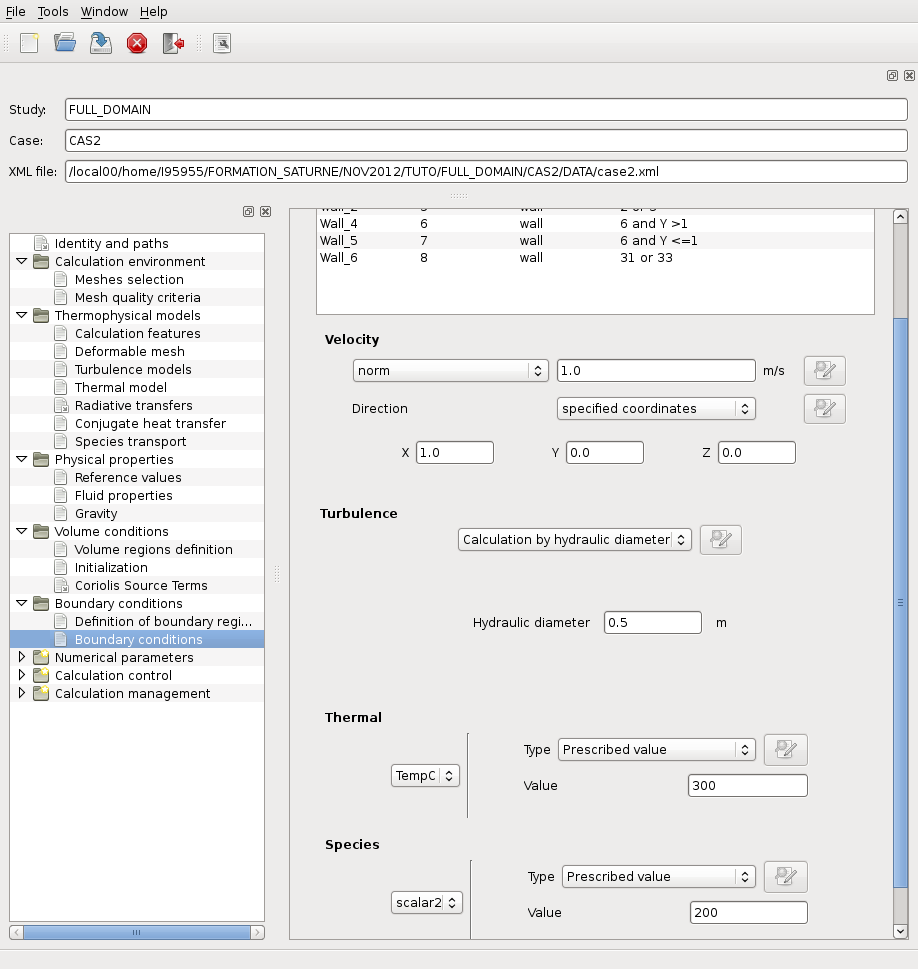
\includegraphics[width=12cm]{case2_V-12}
\caption{Dynamic variables boundary: Inlet}
\end{center}
\end{figure}
\newpage

\fbox{\begin{minipage}{\textwidth}\texttt{
- {\bf Outlet:}
}\end{minipage} }
\begin{figure}[h!]
\begin{center}
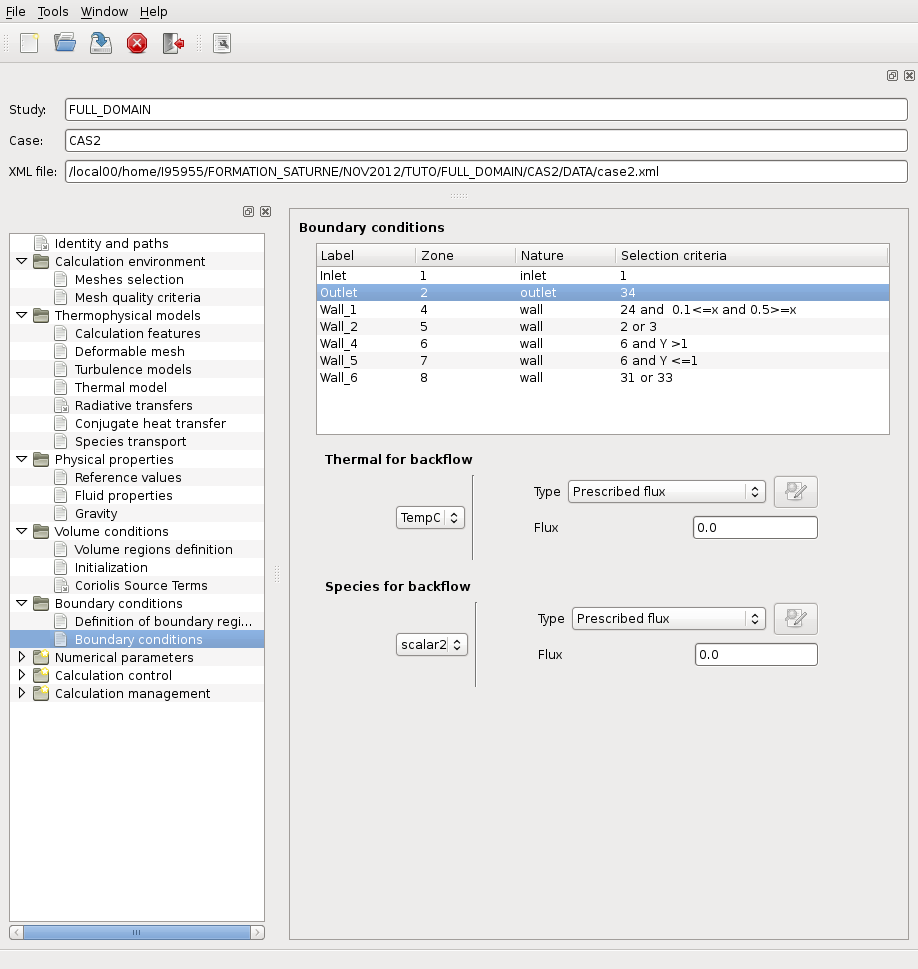
\includegraphics[width=12cm]{case2_V-13}
\caption{Dynamic variables boundary: Outlet}
\end{center}
\end{figure}

\newpage
To configure the scalar boundary conditions on the walls, select individually each
wall in the {\itshape Boundary conditions} item.

On all the walls, a default homogeneous \texttt{prescribed flux} is set for temperature,
and \texttt{prescribed values} are
specified for the passive scalar, named \texttt{scalar2}, according to the following table:\\
\begin{center}
\begin{tabular}{|c|c|c|}
\hline
Wall & Nature & \texttt{Scalar2} value \\
\hline
\hline
wall\_1 & Prescribed value  & 0 \\
\hline
wall\_2 & Prescribed value  & 5 \\
\hline
wall\_3 & Prescribed value  & 0 \\
\hline
wall\_4 & Prescribed value  & 25 \\
\hline
wall\_5 & Prescribed value  & 320 \\
\hline
wall\_6 & Prescribed value  & 40 \\
\hline
\end{tabular}
\end{center}

\begin{figure}[h!]
\begin{center}
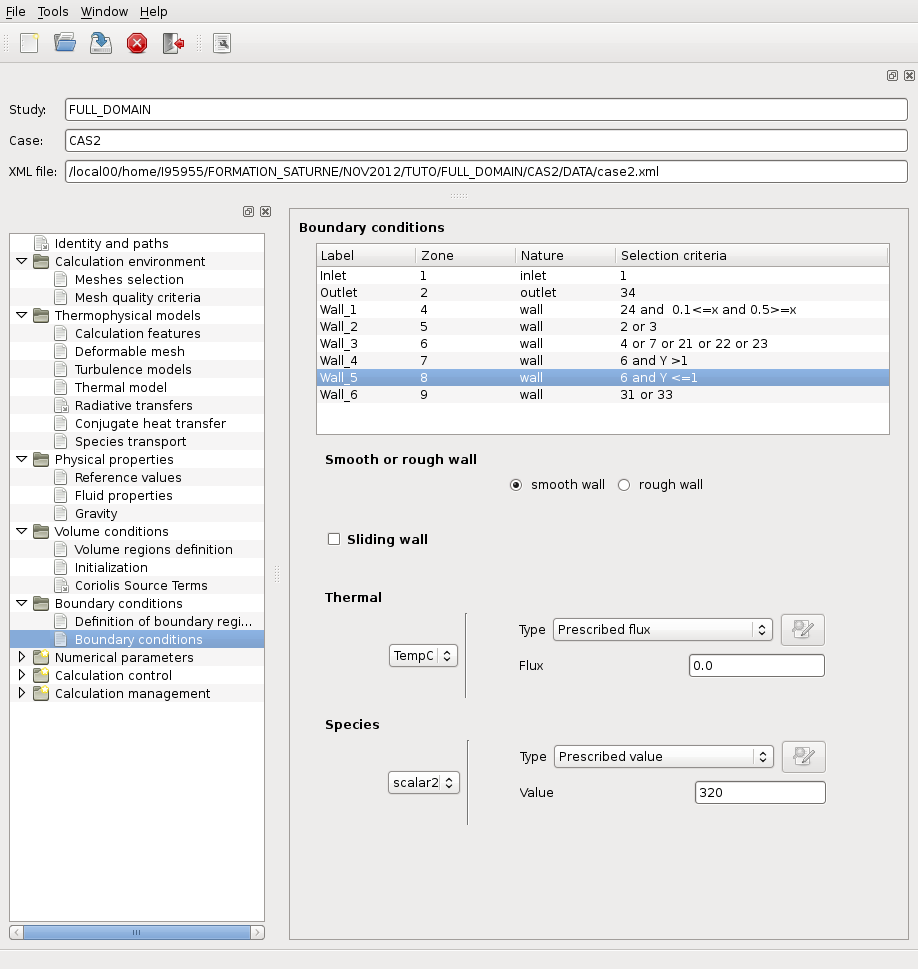
\includegraphics[width=9cm]{case2_V-14}
\caption{Scalars boundaries: wall\_5}
\label{fig21_e2}
\end{center}
\end{figure}

\newpage
Some calculation parameters now need to be defined.
Go to the {\itshape Global parameters} item under the heading
{\itshape Numerical parameters}.
In our case the Pressure-Velocity algorithm is  {\itshape SIMPLEC}.
\begin{figure}[h!]
\begin{center}
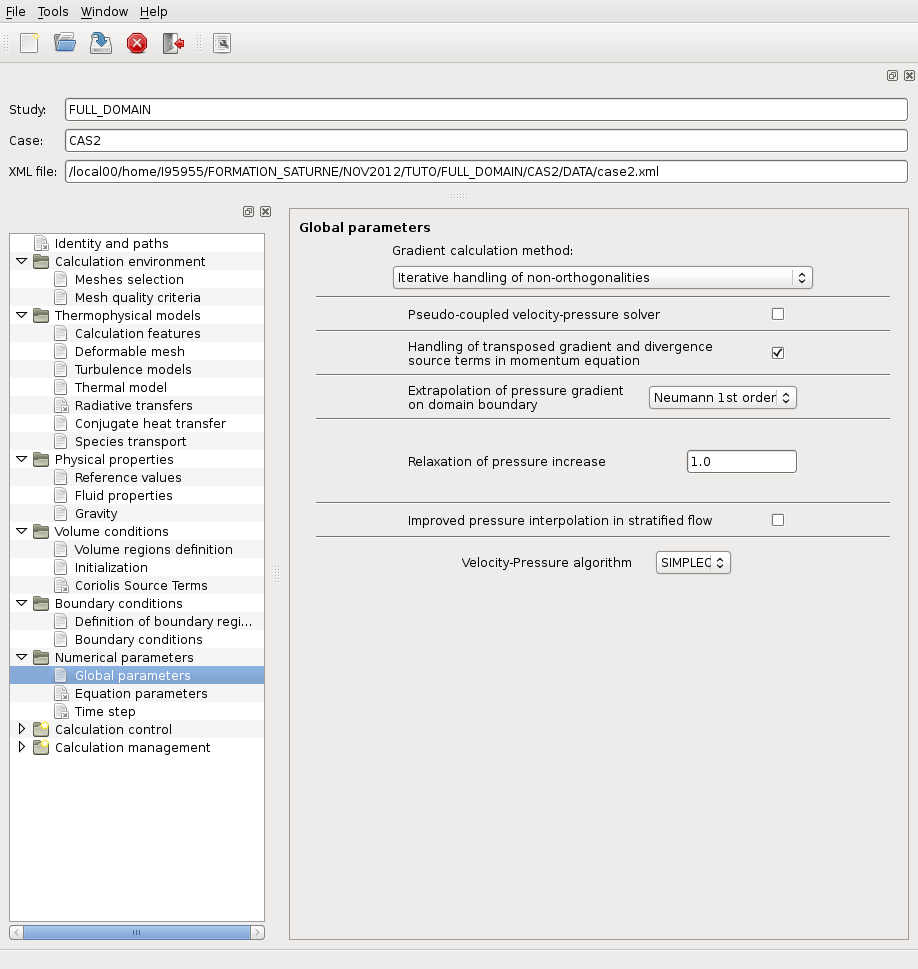
\includegraphics[width=12cm]{case2_V-15}
\caption{Time step setting}
\label{fig23_e2}
\end{center}
\end{figure}

\newpage
Go to the {\itshape Equations parameters} item under the heading
{\itshape Numerical parameters}. You can define the maximum and
minimun value for the \texttt{TempC} and for the \texttt{scalar2} scalars.
\begin{figure}[h!]
\begin{center}
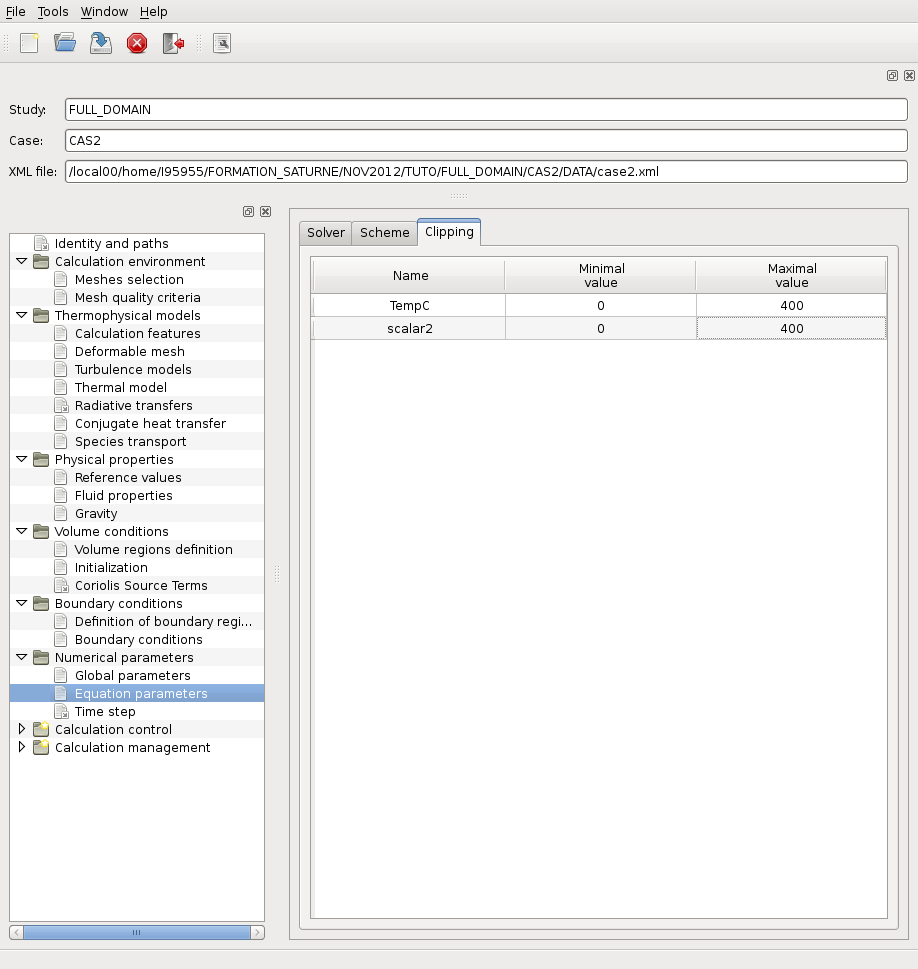
\includegraphics[width=12cm]{case2_V-16}
\caption{Clipping}
\label{fig24_e2}
\end{center}
\end{figure}

\newpage
Go to the {\itshape Time step} item under the heading
{\itshape Numerical parameters}. In our case the time step is
{\itshape Constant}. Set the number of iterations to {\bf 300} and the
reference time step to {\bf 0.05} ($s$).
\begin{figure}[h!]
\begin{center}
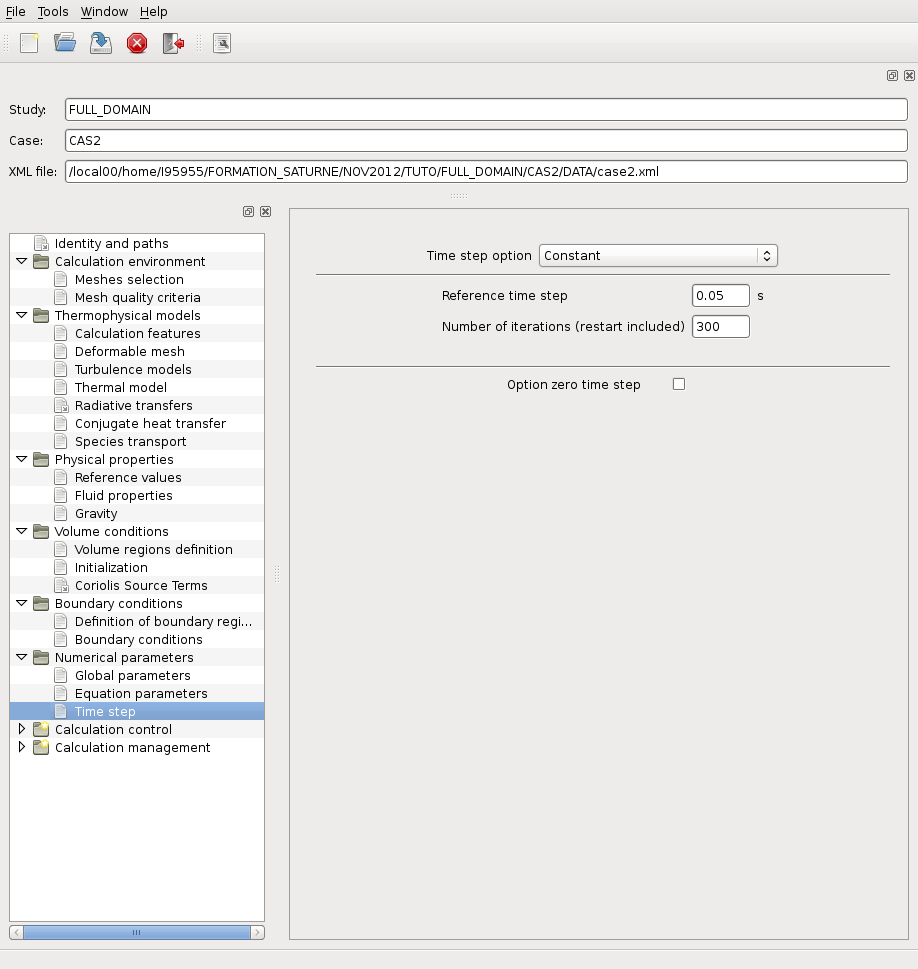
\includegraphics[width=12cm]{case2_V-17}
\caption{Time step setting}
\label{fig24_e2}
\end{center}
\end{figure}

% No change is needed in the {\itshape Equation parameters} and {\itshape Global parameters} items.

\newpage
Go to the {\itshape Output control} item under the heading {\itshape Calculation control} to set the output parameters.
In the {\itshape Output control} item, keep the default value for the output listing frequency.
\begin{figure}[h!]
\begin{center}
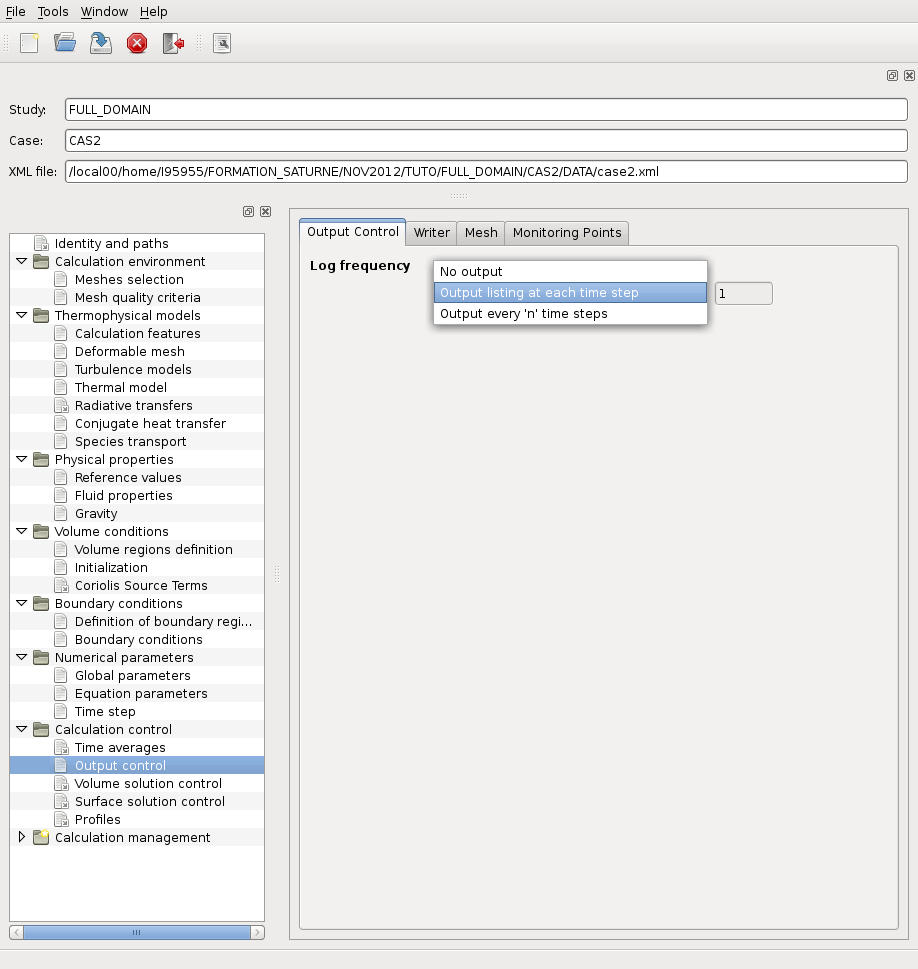
\includegraphics[width=12cm]{case2_V-18}
\caption{Output control: log frequency}
\label{fig23a_e2}
\end{center}
\end{figure}


\newpage
For the Post-processing, go to the {\itshape Writer} item and click on ``results``.
\begin{figure}[h!]
\begin{center}
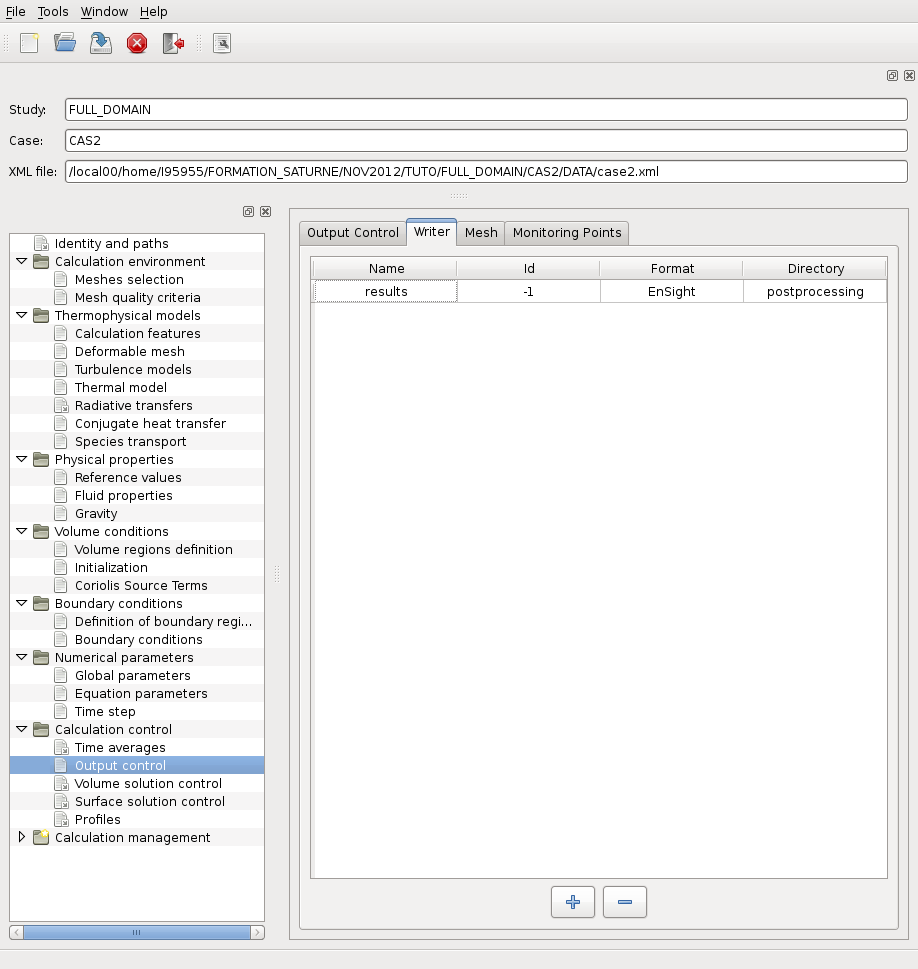
\includegraphics[width=12cm]{case2_V-19}
\caption{Output control: Writer}
\label{fig23b_e2}
\end{center}
\end{figure}
\newpage
Now you can select the third option in the {\itshape Frequency (output every 'n' time steps)} item
and set the value of 'n' to {\bf 2}. By default, the boundary faces are selected.
\begin{figure}[h!]
\begin{center}
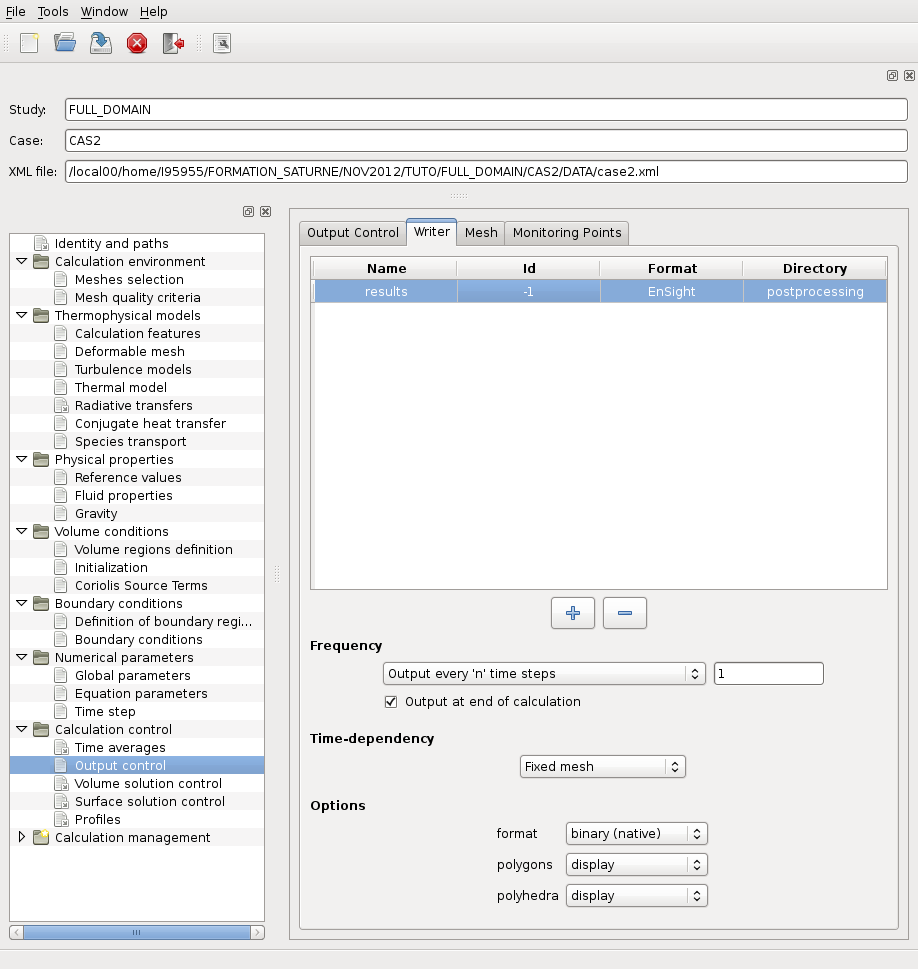
\includegraphics[width=12cm]{case2_V-20}
\caption{Output control: results}
\label{fig23c_e2}
\end{center}
\end{figure}

\newpage

\begin{figure}[h!]
\begin{center}
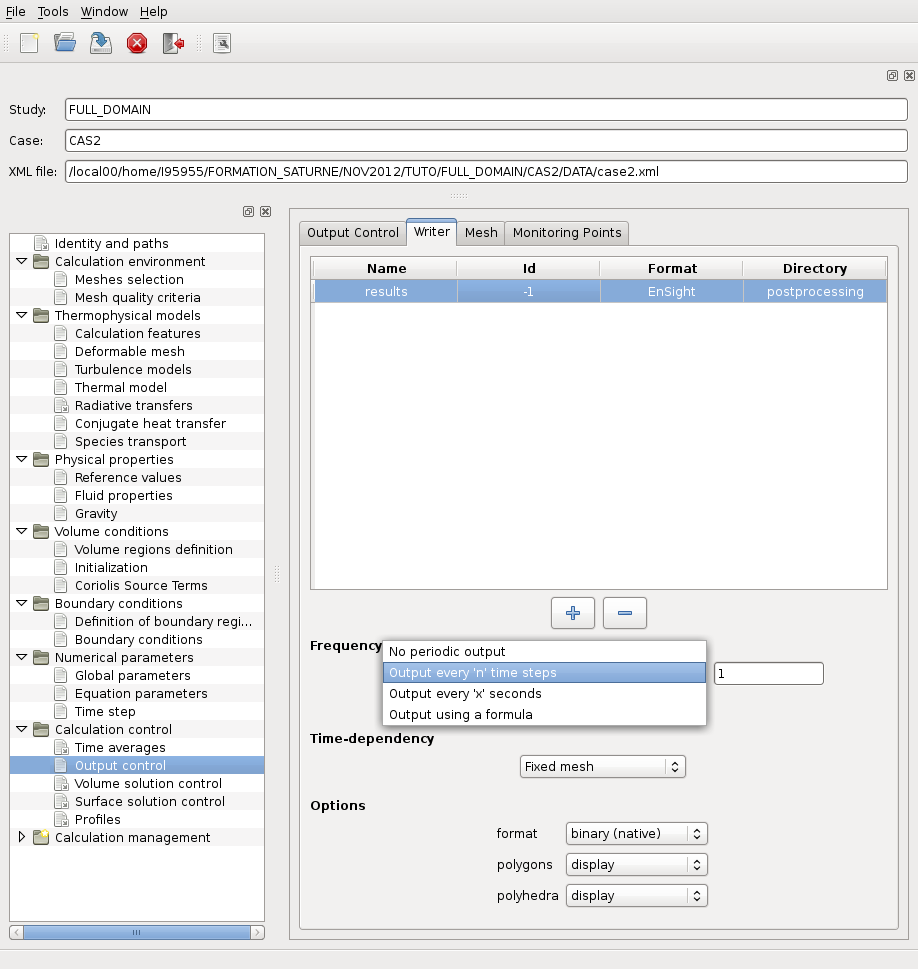
\includegraphics[width=12cm]{case2_V-21}
\caption{Output control: frequency}
\label{fig23d_e2}
\end{center}
\end{figure}

\newpage
You can also choose the format. In this case, you will choose the \ensight format.
\begin{figure}[h!]
\begin{center}
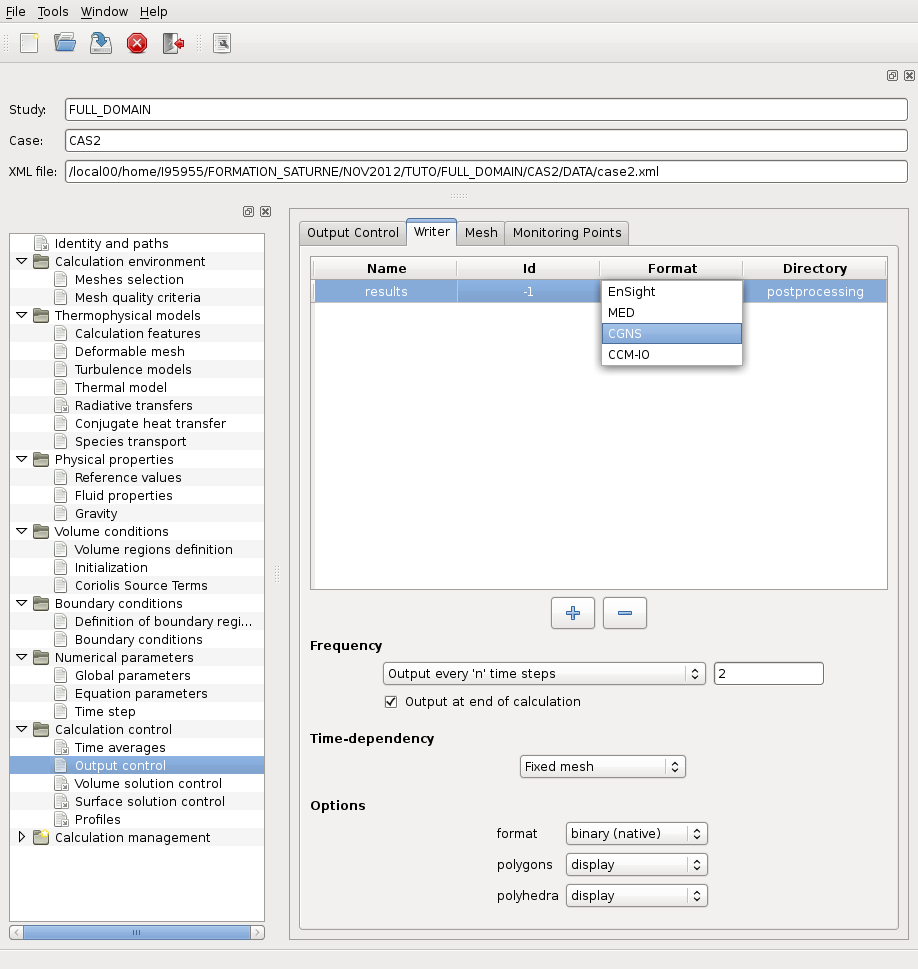
\includegraphics[width=12cm]{case2_V-22}
\caption{Output control: format}
\label{fig23e_e2}
\end{center}
\end{figure}

\newpage

Go to the {\itshape{Mesh}} item.
\begin{figure}[h!]
\begin{center}
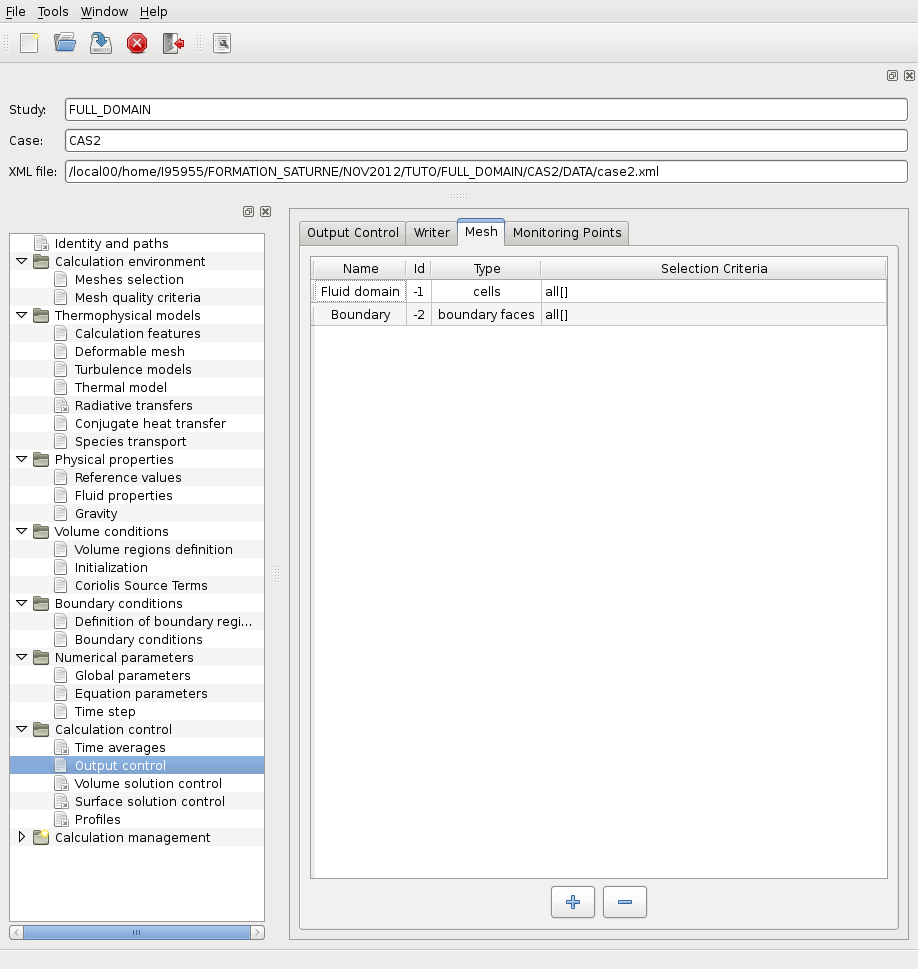
\includegraphics[width=12cm]{case2_V-23}
\caption{Output control: mesh}
\label{fig23f_e2}
\end{center}
\end{figure}

\newpage
You can click on the {\itshape Fluid domain Mesh Name } item and new options will appear.
\begin{figure}[h!]
\begin{center}
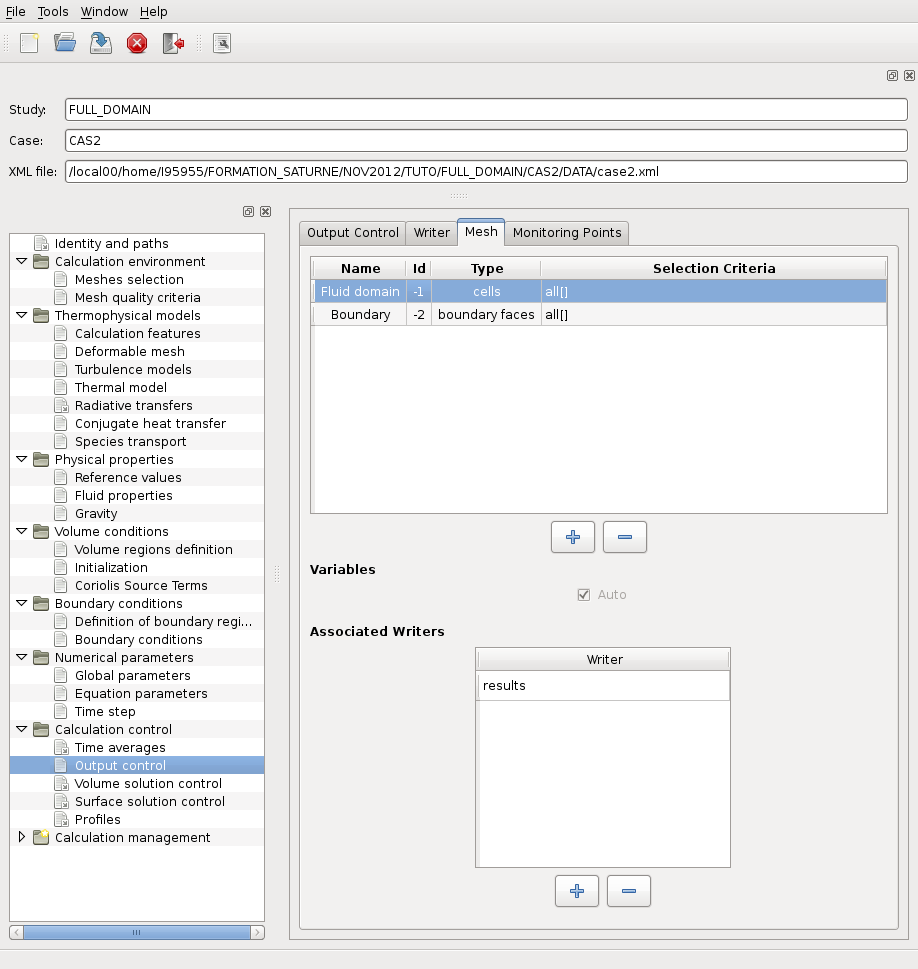
\includegraphics[width=12cm]{case2_V-24}
\caption{Output control: post-processing}
\label{fig24_e2}
\end{center}
\end{figure}

\newpage
You can associated a mesh with several writers.
\begin{figure}[h!]
\begin{center}
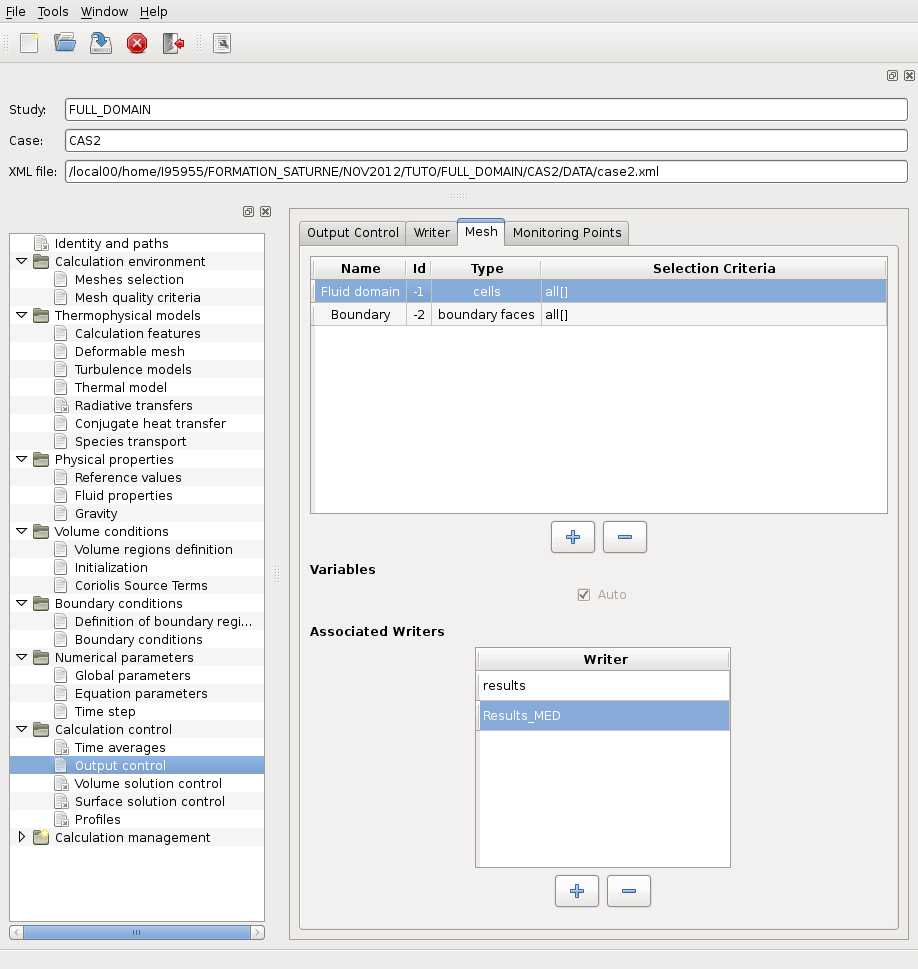
\includegraphics[width=12cm]{case2_V-25}
\caption{Output control:associated writers}
\label{fig24_e2}
\end{center}
\end{figure}

\newpage
In this case, chronological records on specified monitoring probes are needed.
To define the probes, click on the
{\itshape Monitoring points Coordinates} tab.

\begin{figure}[h!]
\begin{center}
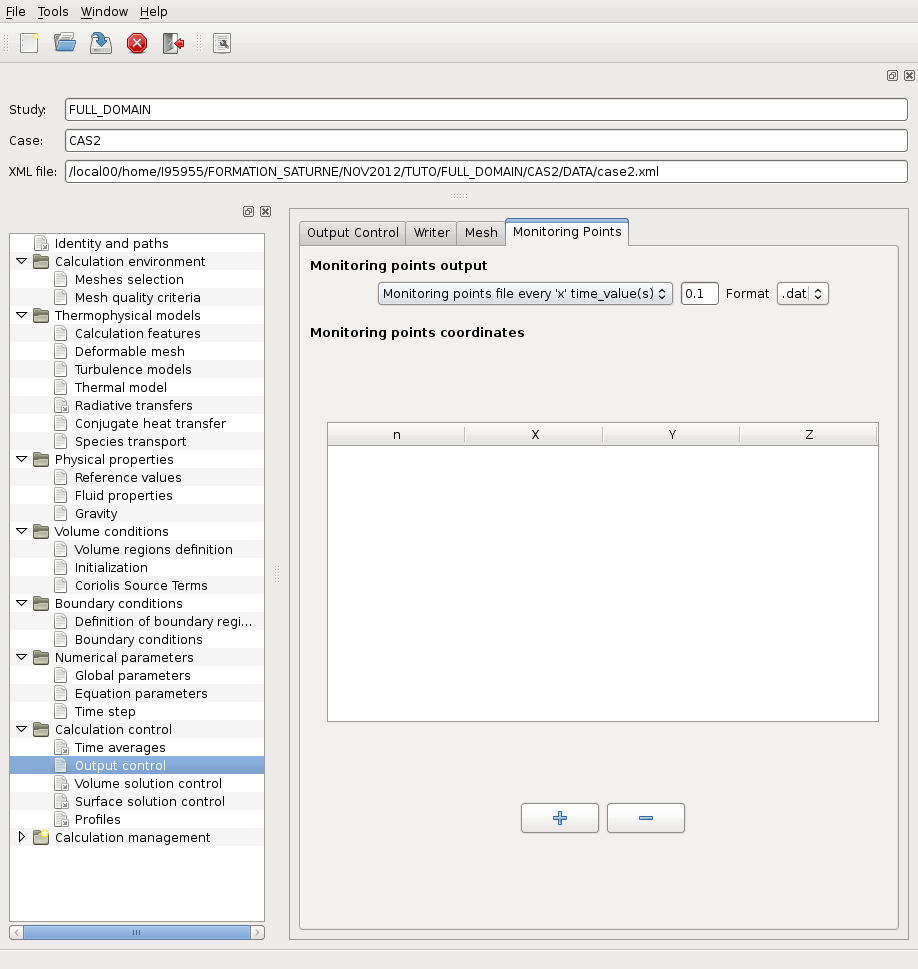
\includegraphics[width=12cm]{case2_V-26}
\caption{Output control: monitoring points}
\label{fig25_e2}
\end{center}
\end{figure}



\newpage
Click on {\bf ``+''} and enter the coordinates of the monitoring points you want to define.

For the first probe:\\
\fbox{\begin{minipage}{\textwidth}\texttt{    \\
 Probe (1) : x = -0.25 (m) ; y = 2.25 (m) ; z = 0.0 (m)
}\end{minipage} }


\begin{figure}[h!]
\begin{center}
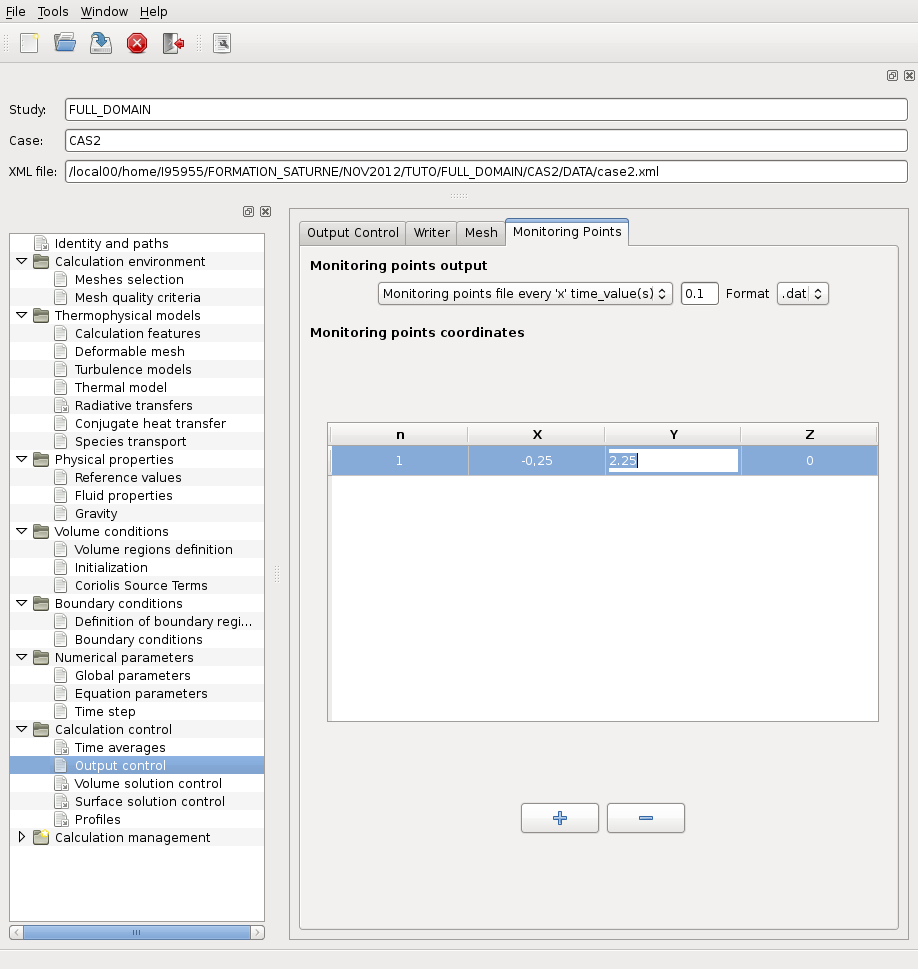
\includegraphics[width=8cm]{case2_V-27}
\caption{Output controls: monitoring points - $1^{st}$ point}
\label{fig27_e2}
\end{center}
\end{figure}


\newpage
Repeat the procedure for the other probes. Their coordinates are indicated in
the following table (the z coordinate is always 0).
\begin{center}
\begin{tabular}{|l|l|l|}
\hline
Probe n$^o$. & x (m) & y (m) \\
\hline
\hline
2 & 0.05 & ~2.25 \\
\hline
3 & 0.05 & ~2.75 \\
\hline
4 & 0.05 & ~0.50 \\
\hline
5 & 0.05 & -0.25 \\
\hline
6 & 0.75 & -0.25 \\
\hline
7 & 0.75 & ~0.25 \\
\hline
8 & 0.75 & ~0.75 \\
\hline
\end{tabular}
\end{center}

\begin{figure}[h!]
\begin{center}
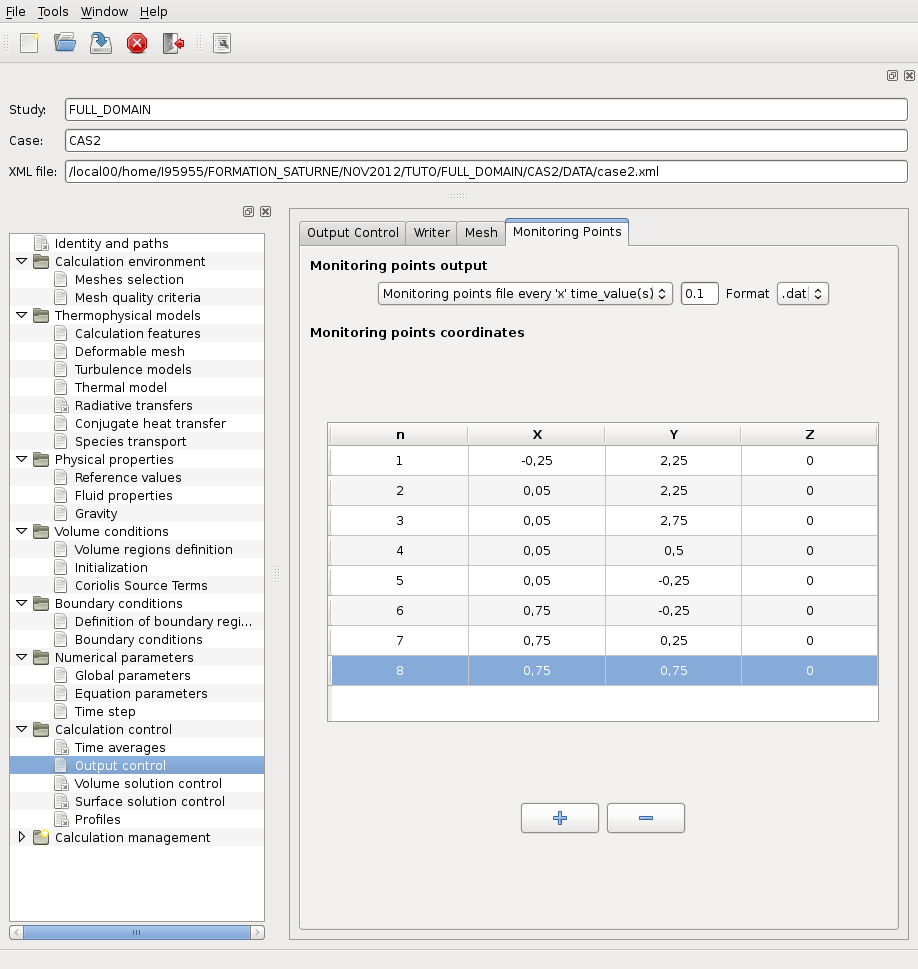
\includegraphics[width=9cm]{case2_V-28}
\caption{Output control: monitoring points}
\label{fig28_e2}
\end{center}
\end{figure}

Remember to save the \texttt{xml} file regularly.


\newpage
Go to the {\itshape Volume solution control} item to define which variables will
appear in the listing, the post-processing and the chronological records.

Uncheck the boxes in front of the {\itshape Pressure}, {\itshape Tubulent Energy}
and {\itshape Dissipation} variables, in the {\itshape  Print in listing} column.
Information on these three variables will not appear in the output listing anymore.

Uncheck the boxes in front of the {\itshape Courant number} and {\itshape Fourier number}
variables in the {\itshape Post-processing} column. These variables will be removed from
the post-processing results.

\begin{figure}[h!]
\begin{center}
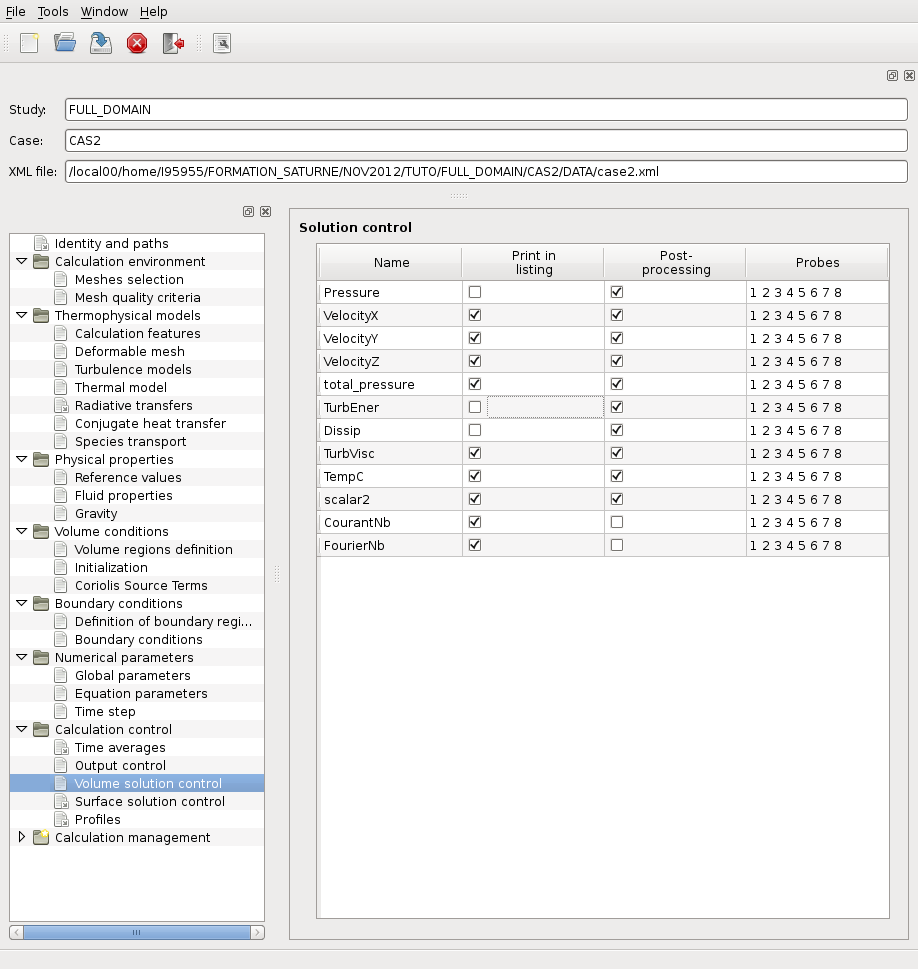
\includegraphics[width=12cm]{case2_V-29}
\caption{Solution control - Output configuration}
\label{fig29_e2}
\end{center}
\end{figure}


\newpage
Delete all the probe numbers for the {\itshape total\_pressure} variable.
No chronological record will be created for this variable.

As for the {\itshape VelocityX} variable, only select probes  1, 2, 6, 7 and 8.
Time evolution on the other probes will not be recorded.

\begin{figure}[h!]
\begin{center}
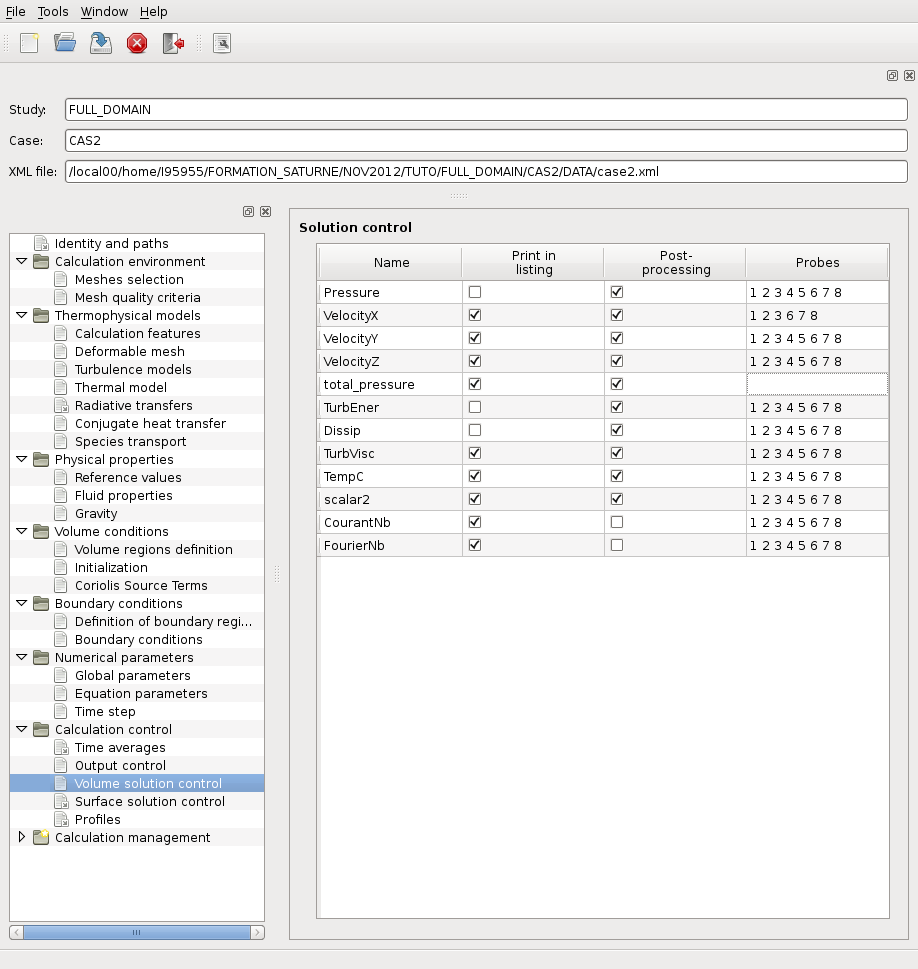
\includegraphics[width=10cm]{case2_V-30}
\caption{Solution control - Probes}
\label{fig30_e2}
\end{center}
\end{figure}

Switch to the {\itshape Calculation management} heading to prepare the launch
script and run the calculation.

